\section{Approximation de l'opérateur d'impédance pour un plan infini par une condition d'impédance d'ordre élevée}

  \subsection{Expression de la condition d'impédance d'ordre élevée}

    On sait que le symbole \(\hat{\mZ}(k_x,k_y)\) s'écrit

    \begin{multline}
        \hat \mZ_m = -k_{3m}
        \left(ik_{3m}\tan\left(k_{3m}d_m\right)\mI - \hat \mZ_{m-1}\mC_m\right) \\
        \left(k_{3m}\mI - i\tan\left(k_{3m}d_m\right)\hat \mZ_{m-1}\mC_m\right)^{-1}
        \mC_m^{-1}
    \end{multline}

    où la matrice \(\mC_m\) est telle que
    \begin{align}
       \mC_m &= \frac{1}{k_m\eta_m}
        \begin{bmatrix}
            k_m^2 - k_y^2 & k_xk_y\\
            k_xk_y & k_m^2 - k_y^2
        \end{bmatrix}
    \end{align}

    Dans le cadre de cette thèse, nous nous intéressons à la condition d'impédance d'\cite{aubakirov_electromagnetic_2014} qui s'exprime en tout point de la surface extérieur de notre objet telle que

    \begin{align}
        \left(I + b_1 \LD{} -b_2 \LR \right)\vE_t = \left(a_0 I + a_1 \LD{} - a_2 \LR \right)(\vn \pvect \vH) & \forall x \in \Gamma
    \end{align}

    Nous la nommons CI3.

    Pour approcher le symbole \(\hat{\mZ}\) que l'on a défini dans l'espace de Fourier, il convient donc d'exprimer les opérateurs \(\LD, \LR\) dans cet espace.

    % Pour cela, nous utiliserons la relation de \cite[Corollary 2,p. ~154]){yosida_functional_1995}:

    Par définition, on a
    \begin{align}
      \LD \vE_t & = \vgrads{} \vdivs{} \vE_t
    \end{align}

    Or

    \begin{align}
      \vE_t(x,y,z) & = \int_\RR\int_\RR \hat{\vE_t}(k_x,k_y,z)e^{ik_xx + ik_yy}\dd{k_x}\dd{k_y}
    \end{align}


    donc

    \begin{align}
      \LD \vE_t
      & = \vgrads{} \vdivs{} \vE_t
      \\
      &=\vgrads{} \int_\RR\int_\RR \hat{\vE_t}(k_x,k_y,z) \cdot \vgrads{} e^{ik_xx + ik_yy}\dd{k_x}\dd{k_y}
      \\
      &=\int_\RR \int_\RR \vhesss{}\left(\left( e^{ik_xx + ik_yy} \right) \hat{\vE_t}\right)(k_x,k_y,z)\dd{k_x}\dd{k_y}
    \end{align}

    On définit \(\hat{\LD}\) l'opérateur matriciel tel que
    \begin{align}
      \LD \vE_t
      &= \int_\RR\int_\RR \hat{\LD} \hat{\vE_t}(k_x,k_y,z)\dd{k_x}\dd{k_y}
    \end{align}

    \begin{equation}
      \hat{\LD}(k_x,k_y) = -
      \begin{bmatrix}
        k_x^2 & k_x k_y
        \\
        k_x k_y & k_y^2
      \end{bmatrix}
    \end{equation}


    Par définition, on a
    \begin{align}
      \LR \vE_t & = \vrots{} \vrots{} \vE_t
    \end{align}

    donc

    \begin{align}
      \LR \vE_t
      & = \vrots{} \vrots{} \vE_t
      \\
      &=\vrots{} \int_\RR\int_\RR \vgrads{}\left(e^{ik_xx + ik_yy}\right) \pvect \hat{\vE_t}(k_x,k_y,z)\dd{k_x}\dd{k_y}
      \\
      &= \int_\RR \int_\RR \left(\vhesss - \vlapls\right) \left(\left(e^{ik_xx + ik_yy}\right) \hat{\vE_t}\right)(k_x,k_y,z)\dd{k_x}\dd{k_y}
      \\
    \end{align}

    On définit \(\hat{\LR}\) l'opérateur matriciel tel que
    \begin{align}
      \LR \vE_t
      &= \int_\RR\int_\RR \hat{\LR} \hat{\vE_t}(k_x,k_y,z)\dd{k_x}\dd{k_y}
    \end{align}

    \begin{equation}
      \hat{\LR}(k_x,k_y) =
      \begin{bmatrix}
        k_y^2 & -k_x k_y
        \\
        -k_x k_y & k_x^2
      \end{bmatrix}
    \end{equation}

    On peut donc définir \(\hat{\mZ}_{IBC}\) l’opérateur matriciel associé à la condition d'impédance.

    \begin{multline}
        \hat{\mZ}_{IBC}(k_x,k_y) = \left(I + b_1 \hat{\LD}(k_x,k_y) - b_2 \hat{\LR}(k_x,k_y) \right)^{-1}
        \\
        \left(a_0 I + a_1 \hat{\LD}(k_x,k_y) - a_2 \hat{\LR}(k_x,k_y)\right)
    \end{multline}

    Pour calculer les coefficients de la CIOE, il faut minimiser la distance entre le symbole \(\hat{\mZ}(k_x,k_y)\) et \(\hat{\mZ}_{IBC}(k_x,k_y)\) \footnote{La distance est la norme de Frobenius}. Évidemment, il existe une infinité de combinaisons pour un couple \((k_x,k_y)\). Nous avons choisis de nous donner un grand nombre de couples et de minimiser au sens des moindres carrés.

    Pour tenir compte d'une onde plane homogène, il faut que \(k_x^2 + k_y^2\) soit inférieur à \(k_0^2\); au delà, nous reproduisons des ondes évanescentes. Nous avons constaté que prendre \(k_x^2 + k_y^2\) inférieur à \(2k_0\) est suffisant pour prendre en compte des ondes guidées dans le cas des matériaux sans pertes.

  \subsection{Le cas spécial de la condition de Leontovich}

    La condition de Leontovich consiste à approcher le symbole par une constante, et donc d'avoir \(a_1=a_2=b_1=b_2=0\). Dans le paragraphe précèdent, cela revient à chercher la valeur moyenne du symbole. Cependant, cette condition rend compte de l'impédance à incidence normale. Dans ce cas particulier, nous ne réaliserons pas de minimisation mais on fixera cette constante à la valeur du symbole en \((0,0)\).

    \begin{equation}
      a_0 = \hat{\mZ}(0,0)
    \end{equation}

  \subsection{Résultats numériques}

      La figure \ref{fig:imp_fourier:plan:hoppe:33:hoibc} permet de vérifier les résultats de \cite[p.~33]{hoppe_impedance_1995} pour une couche de matériau sans perte où il n'y a pas de \(k_x\) réel tel que \(kd=\frac{\pi}{2} + n \pi\) donc pas d'asymptote pour le symbole. La condition d'impédance d'ordre élevé est bien meilleure que la condition de Leontovich.
      \begin{figure}[!hbt]
          \centering
          \tikzsetnextfilename{Z_HOPPE_33_plan_hoibc_TM}
\begin{tikzpicture}[scale=1]
  \begin{axis}[
          title={Polarisation TM},
          ylabel={\(\Im(\hat{Z}(k_x,0)\)},
          xlabel={\(k_x\slash k_0\)},
          width=0.4\textwidth,
          xmin=0,
          xmax=2,
          mark repeat=20,
          legend pos=outer north east
      ]
      \addplot [color=black,mark=square*] table [col sep=comma, x={s1}, y={Im(z_ex.tm)}] {csv/HOPPE_33/HOPPE_33.z_ex.P.csv};
      % \addlegendentry{Exact};

      \addplot [color=blue,mark=x] table [col sep=comma, x={s1}, y={Im(z_ibc0.tm)}] {csv/HOPPE_33/HOPPE_33.z_ibc.IBC_ibc0_TYPE_P_SUC_F.csv};
      % \addlegendentry{CI0};

      \addplot [color=red,mark=diamond*] table [col sep=comma, x={s1}, y={Im(z_ibc3.tm)}] {csv/HOPPE_33/HOPPE_33.z_ibc.IBC_ibc3_TYPE_P_SUC_F.csv};
      % \addlegendentry{CI3};
  \end{axis}
\end{tikzpicture}
\tikzsetnextfilename{Z_HOPPE_33_plan_hoibc_TE}
\begin{tikzpicture}[scale=1]
  \begin{axis}[
          title={Polarisation TE},
          ylabel={},
          xlabel={\(k_x\slash k_0\)},
          width=0.4\textwidth,
          xmin=0,
          xmax=2,
          mark repeat=20,
          legend pos=outer north east
      ]
      \addplot [color=black,mark=square*] table [col sep=comma, x={s1}, y={Im(z_ex.te)}] {csv/HOPPE_33/HOPPE_33.z_ex.P.csv};
      \addlegendentry{Exact};

      \addplot [color=blue,mark=x] table [col sep=comma, x={s1}, y={Im(z_ibc0.te)},color=] {csv/HOPPE_33/HOPPE_33.z_ibc.IBC_ibc0_TYPE_P_SUC_F.csv};
      \addlegendentry{CI0};

      \addplot [color=red,mark=diamond*] table [col sep=comma, x={s1}, y={Im(z_ibc3.te)}] {csv/HOPPE_33/HOPPE_33.z_ibc.IBC_ibc3_TYPE_P_SUC_F.csv};
      \addlegendentry{CI3};
  \end{axis}
\end{tikzpicture}
          \caption[CIOE sur empilement de Hoppe & Rahmat-Samii p.~33]{\(\eps = 4, \mu = 1, d=0.015\text{m}, f=1\text{GHz}\)}
          \label{fig:imp_fourier:plan:hoppe:33:hoibc}
      \end{figure}
      \begin{table}[!hbt]
        \centering
        % On fait deux tables de même hauteur
        \begin{coefftable}{\hyperlink{ci0}{CI0}}
          a_0 & \NaN + \NaN i
          \\
          \\
          \\
          \\
          \\
        \end{coefftable}
        \begin{coefftable}{\hyperlink{ci3}{CI3}}
          a_0 & \NaN + \NaN i
          \\
          a_1 & \NaN + \NaN i
          \\
          a_2 & \NaN + \NaN i
          \\
          b_1 & \NaN + \NaN i
          \\
          b_2 & \NaN + \NaN i
        \end{coefftable}
        \caption{Coefficients associés à la figure \ref{fig:imp_fourier:plan:hoppe:33:hoibc}}
        \label{tab:imp_fourier:plan:hoppe:33:hoibc}
      \end{table}

      La figure \ref{fig:imp_fourier:plan:soudais:hoibc} permet de vérifier les résultats de \cite[p.~11]{soudais_3d_2017} pour une couche de matériau sans perte où il y a une asymptote pour le symbole. La condition d'impédance d'ordre élevé capture cet asymptote grâce à son numérateur et est donc bien meilleure que la condition de Leontovich.
      \begin{figure}[!hbt]
          \centering
          \begin{tikzpicture}[scale=1]
    \begin{axis}[
            title={Polarisation TM},
            ylabel={\(\Im(\hat{Z}(k_x,0)\)},
            xlabel={\(k_x\slash k_0\)},
            width=0.4\textwidth,
            xmin=0,
            xmax=1.8,
            ymin=-1E+1,
            ymax=1E+1,
            restrict y to domain=-30:30,
            mark repeat=40,
            legend pos=outer north east
        ]
        \addplot [color=black,mark=square*] table [col sep=comma, x={s1}, y={Im(z_ex.tm)}] {csv/ICEAA_11/ICEAA_11.z_ex.P.csv};
        % \addlegendentry{Exact};

        \addplot [color=blue,mark=x] table [col sep=comma, x={s1}, y={Im(z_ibc0.tm)}] {csv/ICEAA_11/ICEAA_11.z_ibc.IBC_ibc0_TYPE_P_SUC_F.csv};
        % \addlegendentry{CI0};

        \addplot [color=red,mark=diamond*] table [col sep=comma, x={s1}, y={Im(z_ibc3.tm)}] {csv/ICEAA_11/ICEAA_11.z_ibc.IBC_ibc3_TYPE_P_SUC_F.csv};
        % \addlegendentry{CI3};
    \end{axis}
\end{tikzpicture}
\begin{tikzpicture}[scale=1]
    \begin{axis}[
            title={Polarisation TE},
            ylabel={},
            xlabel={\(k_x\slash k_0\)},
            width=0.4\textwidth,
            xmin=0,
            xmax=1.8,
            ymin=-1E+1,
            ymax=1E+1,
            restrict y to domain=-30:30,
            mark repeat=40,
            legend pos=outer north east
        ]
        \addplot [color=black,mark=square*] table [col sep=comma, x={s1}, y={Im(z_ex.te)}] {csv/ICEAA_11/ICEAA_11.z_ex.P.csv};
        \addlegendentry{Exact};

        \addplot [color=blue,mark=x] table [col sep=comma, x={s1}, y={Im(z_ibc0.te)},color=] {csv/ICEAA_11/ICEAA_11.z_ibc.IBC_ibc0_TYPE_P_SUC_F.csv};
        \addlegendentry{CI0};

        \addplot [color=red,mark=diamond*] table [col sep=comma, x={s1}, y={Im(z_ibc3.te)}] {csv/ICEAA_11/ICEAA_11.z_ibc.IBC_ibc3_TYPE_P_SUC_F.csv};
        \addlegendentry{CI3};
    \end{axis}
\end{tikzpicture}
          \caption[CIOE sur empilement de P.~Soudais p.~11]{Partie imaginaire des coefficients diagonaux de \(\hat\mZ\) pour \(\eps = 4, \mu = 1, d=0.035\text{m}, f=12\text{GHz}\)}
          \label{fig:imp_fourier:plan:soudais:hoibc}
      \end{figure}
      \begin{table}[!hbt]
        \centering
        % On fait deux tables de même hauteur
        \begin{coefftable}{\hyperlink{ci0}{CI0}}
          a_0 & \NaN + \NaN i
          \\
          \\
          \\
          \\
          \\
        \end{coefftable}
        \begin{coefftable}{\hyperlink{ci3}{CI3}}
          a_0 & \NaN + \NaN i
          \\
          a_1 & \NaN + \NaN i
          \\
          a_2 & \NaN + \NaN i
          \\
          b_1 & \NaN + \NaN i
          \\
          b_2 & \NaN + \NaN i
        \end{coefftable}
        \caption{Coefficients associés à la figure \ref{fig:imp_fourier:plan:soudais:hoibc}}
        \label{tab:imp_fourier:plan:soudais:hoibc}
      \end{table}

      On voit sur la figure \ref{fig:reflex_fourier:plan:soudais:hoibc} que cela va de même pour la matrice de réflexion. On déjà vu sur le symbole exact l'onde guidée qui fait diverger ce coefficient de réflexion TM, et on remarque que la CI3 la reproduit assez fidèlement.
      \begin{figure}[!hbt]
          \centering
                    \begin{tikzpicture}[scale=1]
              \begin{axis}[
                      title={Polarisation TM},
                      ylabel={\(|\hat{R}(k_x,0)|\)},
                      xlabel={\(k_x\slash k_0\)},
                      width=0.4\textwidth,
                      ymin=0,
                      ymax=+3E+01,
                      restrict y to domain=0:+4E+01,
                      xmin=0,
                      xmax=1.8,
                      mark repeat=40,
                      legend pos=outer north east
                  ]
                  \addplot [color=black,mark=square*] table [col sep=comma, x={s1}, y={Abs(r_ex.tm)}] {csv/ICEAA_11/ICEAA_11.r_ex.P.csv};
                  % \addlegendentry{Exact};

                  \addplot [color=blue,mark=x] table [col sep=comma, x={s1}, y={Abs(r_ibc0.tm)}] {csv/ICEAA_11/ICEAA_11.r_ibc.IBC_ibc0_TYPE_P_SUC_F.csv};
                  % \addlegendentry{CI0};

                  \addplot [color=red,mark=diamond*] table [col sep=comma, x={s1}, y={Abs(r_ibc3.tm)}] {csv/ICEAA_11/ICEAA_11.r_ibc.IBC_ibc3_TYPE_P_SUC_F.csv};
                  % \addlegendentry{CI3};
              \end{axis}
          \end{tikzpicture}
          \begin{tikzpicture}[scale=1]
              \begin{axis}[
                      title={Polarisation TE},
                      ylabel={},
                      xlabel={\(k_x\slash k_0\)},
                      width=0.4\textwidth,
                      xmin=0,
                      xmax=1.8,
                      ymin=0,
                      ymax=+3E+01,
                      mark repeat=40,
                      legend pos=outer north east
                  ]
                  \addplot [color=black,mark=square*] table [col sep=comma, x={s1}, y={Abs(r_ex.te)}] {csv/ICEAA_11/ICEAA_11.r_ex.P.csv};
                  \addlegendentry{Exact};

                  \addplot [color=blue,mark=x] table [col sep=comma, x={s1}, y={Abs(r_ibc0.te)},color=] {csv/ICEAA_11/ICEAA_11.r_ibc.IBC_ibc0_TYPE_P_SUC_F.csv};
                  \addlegendentry{CI0};

                  \addplot [color=red,mark=diamond*] table [col sep=comma, x={s1}, y={Abs(r_ibc3.te)}] {csv/ICEAA_11/ICEAA_11.r_ibc.IBC_ibc3_TYPE_P_SUC_F.csv};
                  \addlegendentry{CI3};
              \end{axis}
          \end{tikzpicture}
          \caption[CIOE sur empilement de P.~Soudais p.~11]{Module des coefficients diagonaux de \(\mR\) pour \(\eps = 4, \mu = 1, d=0.035\text{m}, f=12\text{GHz}\)}
          \label{fig:reflex_fourier:plan:soudais:hoibc}
      \end{figure}

      La figure \ref{fig:imp_fourier:plan:triple_asymptote:hoibc} montre la limite de la CI3 pour capturer 3 asymptotes. Pour cela, il faudrait utiliser une CI d'ordre au moins 6.

      L'expression de cette CIOE que l'on nomme \hyperlink{ci7}{CI7} est
      \begin{equation}
        \left(\oI + \sum_{i=1}^3 \left(d_{i} \frac{\LD^i}{k_0^2} + e_{i} \frac{(-\LR)^i}{k_0^2} \right)\right)\vE_t = \left(a_0 \oI + \sum_{i=1}^3 \left(b_{i} \frac{\LD^i}{k_0^2} + c_{i} \frac{(-\LR)^i}{k_0^2} \right)\right)\vJ
      \end{equation}

      \begin{figure}[!hbt]
          \centering
          \tikzsetnextfilename{Z_triple_asymptote_plan_hoibc.TM}
\begin{tikzpicture}[scale=1]
    \begin{axis}[
            title={Polarisation TM},
            ylabel={\(\Im(\hat{Z}(k_x,0)\)},
            xlabel={\(k_x\slash k_0\)},
            width=0.4\textwidth,
            xmin=0,
            xmax=1.999,
            ymin=-10,
            ymax=10,
            restrict y to domain=-300:300,
            mark repeat=200,
            legend pos=outer north east
        ]
        \addplot [color=black,mark=square*] table [col sep=comma, x={s1}, y={Im(z_ex.tm)}] {csv/triple_asymptote/triple_asymptote.z_ex.MODE_2_TYPE_P.csv};
        % \addlegendentry{Exact};

        \addplot [color=blue,mark=x] table [col sep=comma, x={s1}, y={Im(z_ibc0.tm)}] {csv/triple_asymptote/triple_asymptote.z_ibc.IBC_ibc0_SUC_F_MODE_2_TYPE_P.csv};
        % \addlegendentry{CI0};

        \addplot [color=red,mark=diamond*] table [col sep=comma, x={s1}, y={Im(z_ibc3.tm)}] {csv/triple_asymptote/triple_asymptote.z_ibc.IBC_ibc3_SUC_F_MODE_2_TYPE_P.csv};
        % \addlegendentry{CI3};

        \addplot [color=cyan,mark=pentagon*] table [col sep=comma, x={s1}, y={Im(z_ibc7.tm)}] {csv/triple_asymptote/triple_asymptote.z_ibc.IBC_ibc7_SUC_F_MODE_2_TYPE_P.csv};
        % \addlegendentry{CI7};
    \end{axis}
\end{tikzpicture}
\tikzsetnextfilename{Z_triple_asymptote_plan_hoibc.TE}
\begin{tikzpicture}[scale=1]
    \begin{axis}[
            title={Polarisation TE},
            ylabel={},
            xlabel={\(k_x\slash k_0\)},
            width=0.4\textwidth,
            xmin=0,
            xmax=1.999,
            ymin=-10,
            ymax=10,
            restrict y to domain=-300:300,
            mark repeat=200,
            legend pos=outer north east
        ]
        \addplot [color=black,mark=square*] table [col sep=comma, x={s1}, y={Im(z_ex.te)}] {csv/triple_asymptote/triple_asymptote.z_ex.MODE_2_TYPE_P.csv};
        \addlegendentry{Exact};

        \addplot [color=blue,mark=x] table [col sep=comma, x={s1}, y={Im(z_ibc0.te)}] {csv/triple_asymptote/triple_asymptote.z_ibc.IBC_ibc0_SUC_F_MODE_2_TYPE_P.csv};
        \addlegendentry{CI0};

        \addplot [color=red,mark=diamond*] table [col sep=comma, x={s1}, y={Im(z_ibc3.te)}] {csv/triple_asymptote/triple_asymptote.z_ibc.IBC_ibc3_SUC_F_MODE_2_TYPE_P.csv};
        \addlegendentry{CI3};

        \addplot [color=cyan,mark=pentagon*] table [col sep=comma, x={s1}, y={Im(z_ibc7.te)}] {csv/triple_asymptote/triple_asymptote.z_ibc.IBC_ibc7_SUC_F_MODE_2_TYPE_P.csv};
        \addlegendentry{CI7};                  
    \end{axis}
\end{tikzpicture}
          \caption[CIOE sur empilement avec triple asymptote]{Partie imaginaire des coefficients diagonaux de \(\mZ\) pour \(\eps = 4, \mu = 1, d=0.2\text{m}, f=1\text{GHz}\)}
          \label{fig:imp_fourier:plan:triple_asymptote:hoibc}
      \end{figure}
      \begin{table}[!hbt]
        \centering
        % On fait deux tables de même hauteur
        \begin{coefftable}{\hyperlink{ci0}{CI0}}
          a_0 & \NaN + \NaN i
          \\
          \\
          \\
          \\
          \\
          \\
          \\
          \\
          \\
          \\
          \\
          \\
          \\
        \end{coefftable}
        \begin{coefftable}{\hyperlink{ci3}{CI3}}
          a_0 & \NaN + \NaN i
          \\
          a_1 & \NaN + \NaN i
          \\
          a_2 & \NaN + \NaN i
          \\
          b_1 & \NaN + \NaN i
          \\
          b_2 & \NaN + \NaN i
          \\
          \\
          \\
          \\
          \\
          \\
          \\
          \\
          \\
        \end{coefftable}
        \begin{coefftable}{\hyperlink{ci7}{CI7}}
          a_0 & \NaN + \NaN i
          \\
          b_1 & \NaN + \NaN i
          \\
          c_1 & \NaN + \NaN i
          \\
          d_1 & \NaN + \NaN i
          \\
          e_1 & \NaN + \NaN i
          \\
          b_2 & \NaN + \NaN i
          \\
          c_2 & \NaN + \NaN i
          \\
          d_2 & \NaN + \NaN i
          \\
          e_2 & \NaN + \NaN i
          \\
          b_3 & \NaN + \NaN i
          \\
          c_3 & \NaN + \NaN i
          \\
          e_3 & \NaN + \NaN i
          \\
          e_3 & \NaN + \NaN i
        \end{coefftable}
        \caption{Coefficients associés à la figure \ref{fig:imp_fourier:plan:triple_asymptote:hoibc}}
        \label{tab:imp_fourier:plan:triple_asymptote:hoibc}
      \end{table}
      Il faut donc une CIOE d'ordre 2 fois le nombre d'asymptote que l'on rencontre sur notre balayage.


  \subsection{Lien avec les CIOE de \cite{stupfel_implementation_2015}}

    Dans cet article sont introduites les CIOE
    \begin{itemize}
      \item CI01
        \begin{equation}
          \vE_t = \left(a_0\oI + a_1\LL\right)\vJ
        \end{equation}
      \item CI1
        \begin{equation}
          \left(\oI + b\LL \right)\vE_t = \left(a_0\oI + a_1\LL\right)\vJ
        \end{equation}
    \end{itemize}

    L'opérateur \(\LL\) est le laplacien tangentiel \(\lapls\) appliqué à chaque composante. Le multiplicateur de Fourier associé est la matrice
    \begin{equation}
      \hat{\mL}  = -
      \begin{bmatrix}
        k_x^2 + k_y^2 & 0
        \\
        0 & k_x^2 + k_y^2
      \end{bmatrix}
    \end{equation}

    Le multiplicateur est multiple de l'identité ce qui en fait un mauvais candidat convenu de la nature diagonale mais non multiple de l’identité du symbole. La figure \ref{fig:imp_fourier:plan:stupfel:hoibc} présente donc quelques résultats où l'on voit bien la limite de ces CIOE.
    \begin{figure}[!hbt]
      \centering
      \begin{tikzpicture}[scale=1]
    \begin{axis}[
            title={Polarisation TM},
            ylabel={\(|\hat{Z}(k_x,0)|\)},
            xlabel={\(k_x\slash k_0\)},
            width=0.4\textwidth,
            xmin=0,
            xmax=1.5,
            ymin=0.15,
            ymax=0.25,
            restrict y to domain=0:11,
            mark repeat=10,
            legend pos=outer north east
        ]
        \addplot [color=black,mark=square*] table [col sep=comma, x={s1}, y={Abs(z_ex.tm)}] {csv/M1/M1.z_ex.P.csv};

        \addplot [color=blue,mark=x] table [col sep=comma, x={s1}, y={Abs(z_ibc0.tm)}] {csv/M1/M1.z_ibc.IBC_ibc0_TYPE_P_SUC_F.csv};

        \addplot [color=green!50!black,mark=pentagon*] table [col sep=comma, x={s1}, y={Abs(z_ibc01.tm)}] {csv/M1/M1.z_ibc.IBC_ibc01_TYPE_P_SUC_F.csv};

        \addplot [color=orange,mark=*] table [col sep=comma, x={s1}, y={Abs(z_ibc1.tm)}] {csv/M1/M1.z_ibc.IBC_ibc1_TYPE_P_SUC_F.csv};

        \addplot [color=red,mark=diamond*] table [col sep=comma, x={s1}, y={Abs(z_ibc3.tm)}] {csv/M1/M1.z_ibc.IBC_ibc3_TYPE_P_SUC_F.csv};
    \end{axis}
\end{tikzpicture}
\begin{tikzpicture}[scale=1]
    \begin{axis}[
            title={Polarisation TE},
            ylabel={},
            xlabel={\(k_x\slash k_0\)},
            width=0.4\textwidth,
            xmin=0,
            xmax=1.5,
            ymin=0.15,
            ymax=0.25,
            mark repeat=10,
            restrict y to domain=0:11,
            legend pos=outer north east
        ]
        \addplot [color=black,mark=square*] table [col sep=comma, x={s1}, y={Abs(z_ex.te)}] {csv/M1/M1.z_ex.P.csv};
        \addlegendentry{Exact};

        \addplot [color=blue,mark=x] table [col sep=comma, x={s1}, y={Abs(z_ibc0.te)},color=] {csv/M1/M1.z_ibc.IBC_ibc0_TYPE_P_SUC_F.csv};
        \addlegendentry{CI0};

        \addplot [color=green!50!black,mark=pentagon*] table [col sep=comma, x={s1}, y={Abs(z_ibc01.te)}] {csv/M1/M1.z_ibc.IBC_ibc01_TYPE_P_SUC_F.csv};
        \addlegendentry{CI01};

        \addplot [color=orange,mark=*] table [col sep=comma, x={s1}, y={Abs(z_ibc1.te)}] {csv/M1/M1.z_ibc.IBC_ibc1_TYPE_P_SUC_F.csv};
        \addlegendentry{CI1};

        \addplot [color=red,mark=diamond*] table [col sep=comma, x={s1}, y={Abs(z_ibc3.te)}] {csv/M1/M1.z_ibc.IBC_ibc3_TYPE_P_SUC_F.csv};
        \addlegendentry{CI3};

    \end{axis}
\end{tikzpicture}
      \caption[CIOE sur empilement de B.~Stupfel p.~1661]{Module des coefficients diagonaux de \(\hat\mZ\) pour \(\eps = 1-i, \mu = 1, d=0.05\text{m}, f=0.2\text{GHz}\)}
      \label{fig:imp_fourier:plan:stupfel:hoibc}
    \end{figure}
      \begin{table}[!hbt]
        \centering
        % On fait deux tables de même hauteur
        \begin{coefftable}{\hyperlink{ci0}{CI0}}
          a_0 & \NaN + \NaN i
          \\
          \\
        \end{coefftable}
        \begin{coefftable}{\hyperlink{ci01}{CI01}}
          a_0 & \NaN + \NaN i
          \\
          a_1 & \NaN + \NaN i
        \end{coefftable}

        \begin{coefftable}{\hyperlink{ci1}{CI1}}
          a_0 & \NaN + \NaN i
          \\
          a_1 & \NaN + \NaN i
          \\
          b  & \NaN + \NaN i
          \\
          \\
          \\
        \end{coefftable}
        \begin{coefftable}{\hyperlink{ci3}{CI3}}
          a_0 & \NaN + \NaN i
          \\
          a_1 & \NaN + \NaN i
          \\
          a_2 & \NaN + \NaN i
          \\
          b_1 & \NaN + \NaN i
          \\
          b_2 & \NaN + \NaN i
        \end{coefftable}
        \caption{Coefficients associés à la figure \ref{fig:imp_fourier:plan:stupfel:hoibc}}
        \label{tab:imp_fourier:plan:stupfel:hoibc}
      \end{table}
    \begin{figure}[!hbt]
      \centering
      \tikzsetnextfilename{R_cioe_2015_plan_hoibc_TM}
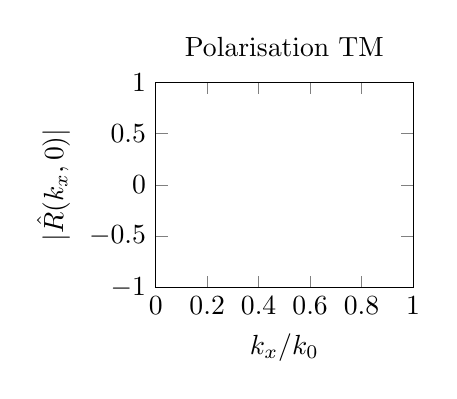
\begin{tikzpicture}[scale=1]
    \begin{axis}[
            title={Polarisation TM},
            ylabel={\(|\hat{R}(k_x,0)|\)},
            xlabel={\(k_x\slash k_0\)},
            width=0.4\textwidth,
            xmin=0,
            xmax=1,
            ymin=-1,
            ymax=1,
            mark repeat=15,
            legend pos=outer north east
        ]
        % \addplot [color=black,mark=square*] table [col sep=comma, x={s1}, y={Abs(r_ex.tm)}] {csv/STUPFEL/STUPFEL.r_ex.MODE_2_TYPE_P.csv};

        % \addplot [color=blue,mark=x] table [col sep=comma, x={s1}, y={Abs(r_ibc0.tm)}] {csv/STUPFEL/STUPFEL.r_ibc.IBC_ibc0_SUC_F_MODE_2_TYPE_P.csv};

        % \addplot [color=green!50!black,mark=pentagon*] table [col sep=comma, x={s1}, y={Abs(r_ibc01.tm)}] {csv/STUPFEL/STUPFEL.r_ibc.IBC_ibc01_SUC_F_MODE_2_TYPE_P.csv};

        % \addplot [color=orange,mark=*] table [col sep=comma, x={s1}, y={Abs(r_ibc1.tm)}] {csv/STUPFEL/STUPFEL.r_ibc.IBC_ibc1_SUC_F_MODE_2_TYPE_P.csv};

        % \addplot [color=red,mark=diamond*] table [col sep=comma, x={s1}, y={Abs(r_ibc3.tm)}] {csv/STUPFEL/STUPFEL.r_ibc.IBC_ibc3_SUC_F_MODE_2_TYPE_P.csv};
    \end{axis}
\end{tikzpicture}
\tikzsetnextfilename{R_cioe_2015_plan_hoibc_TE}
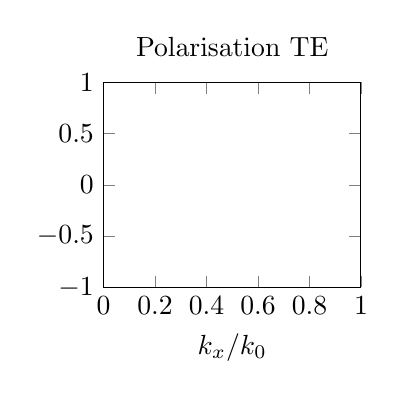
\begin{tikzpicture}[scale=1]
    \begin{axis}[
            title={Polarisation TE},
            ylabel={},
            xlabel={\(k_x\slash k_0\)},
            width=0.4\textwidth,
            xmin=0,
            xmax=1,
            ymin=-1,
            ymax=1,
            mark repeat=15,
            legend pos=outer north east
        ]
        % \addplot [color=black,mark=square*] table [col sep=comma, x={s1}, y={Abs(r_ex.te)}] {csv/STUPFEL/STUPFEL.r_ex.MODE_2_TYPE_P.csv};
        % \addlegendentry{Exact};

        % \addplot [color=blue,mark=x] table [col sep=comma, x={s1}, y={Abs(r_ibc0.te)},color=] {csv/STUPFEL/STUPFEL.r_ibc.IBC_ibc0_SUC_F_MODE_2_TYPE_P.csv};
        % \addlegendentry{CI0};

        % \addplot [color=green!50!black,mark=pentagon*] table [col sep=comma, x={s1}, y={Abs(r_ibc01.te)}] {csv/STUPFEL/STUPFEL.r_ibc.IBC_ibc01_SUC_F_MODE_2_TYPE_P.csv};
        % \addlegendentry{CI01};

        % \addplot [color=orange,mark=*] table [col sep=comma, x={s1}, y={Abs(r_ibc1.te)}] {csv/STUPFEL/STUPFEL.r_ibc.IBC_ibc1_SUC_F_MODE_2_TYPE_P.csv};
        % \addlegendentry{CI1};

        % \addplot [color=red,mark=diamond*] table [col sep=comma, x={s1}, y={Abs(r_ibc3.te)}] {csv/STUPFEL/STUPFEL.r_ibc.IBC_ibc3_SUC_F_MODE_2_TYPE_P.csv};
        % \addlegendentry{CI3};

    \end{axis}
\end{tikzpicture}
      \caption[CIOE sur empilement de B.~Stupfel p.~1661]{Module des coefficients diagonaux de \(\mR\) pour \(\eps = 1-i, \mu = 1, d=0.05\text{m}, f=0.2\text{GHz}\)}
      \label{fig:reflex_fourier:plan:stupfel:hoibc}
    \end{figure}